\documentclass[12pt,a4paper]{article}

\usepackage[utf8]{inputenc}
\usepackage[T1]{fontenc}
\usepackage[french]{babel}
\usepackage{geometry}
\usepackage{graphicx}
\usepackage{booktabs}
\usepackage{longtable}
\usepackage{array}
\usepackage{xcolor}
\usepackage{hyperref}
\usepackage{listings}
\usepackage{enumitem}
\usepackage{titlesec}
\usepackage{fancyhdr}
\usepackage{multirow}
\usepackage{float}

\geometry{margin=2.5cm}

\definecolor{bronze}{RGB}{205,127,50}
\definecolor{silver}{RGB}{160,160,160}
\definecolor{gold}{RGB}{212,175,55}
\definecolor{codeblue}{RGB}{0,100,180}
\definecolor{codegray}{RGB}{245,245,245}

\lstset{
  backgroundcolor=\color{codegray},
  basicstyle=\ttfamily\small,
  breaklines=true,
  frame=single,
  rulecolor=\color{gray}
}

\pagestyle{fancy}
\fancyhf{}
\lhead{\small Observatoire immobilier -- Clé en Main Immo}
\rhead{\small Warehousing, Data Lakes \& Polystores}
\cfoot{\thepage}
\renewcommand{\headrulewidth}{0.5pt}

\hypersetup{colorlinks=true,linkcolor=codeblue,urlcolor=codeblue}

\graphicspath{{diagrams/}}

\begin{document}

% -------------------------------------------------------
%  Page de titre
% -------------------------------------------------------
\begin{titlepage}
  \centering
  \vspace*{2cm}
  {\Large Université de Blois\par}
  \vspace{0.3cm}
  {\large Master 2 Data Science for Societal Challenges (DS4SC)\par}
  \vspace{1.5cm}
  \noindent\rule{\linewidth}{1.5pt}
  \vspace{0.6cm}

  {\Huge\bfseries Observatoire immobilier --- Data Lake\par}
  \vspace{0.4cm}
  {\Large Clé en Main Immo\par}

  \vspace{0.6cm}
  \noindent\rule{\linewidth}{1.5pt}
  \vspace{1cm}

  {\large Warehousing, Data Lakes \& Polystores --- Groupe 4\par}

  \vspace{2.5cm}
  {\normalsize\bfseries Étudiants~:\par}
  \vspace{0.3cm}
  {\normalsize
    Rayan HACHEMI\\
    Leiticia ARIB\\
    Ouissam BOUZID\\
    Mehdi IMLOUL\par
  }

  \vspace{1.2cm}
  {\normalsize\bfseries Encadrants~:\par}
  \vspace{0.3cm}
  {\normalsize
    Alexandre Chanson\\
    Hassan Abdallah\par
  }

  \vfill
  {\normalsize Novembre 2026\par}
\end{titlepage}

\tableofcontents
\newpage

% -------------------------------------------------------
%  1. Introduction
% -------------------------------------------------------
\section{Introduction et contexte métier}

Ce projet a pour objectif la conception, la modélisation et l'implémentation d'un Data Lake
permettant l'intégration et la préparation de données hétérogènes, dans le cadre du cours
\textit{Warehousing, Data Lakes \& Polystores} du Master 2 DS4SC de l'Université de Blois.

\subsection{Cas d'usage}

Le client fictif est l'agence immobilière \textbf{Clé en Main Immo}, qui souhaite disposer
d'un observatoire automatisé pour répondre à cinq besoins métier~:

\begin{itemize}[noitemsep]
  \item \textbf{B1} -- Argumentaire de prix en temps réel pour un bien visité
  \item \textbf{B2} -- Score de potentiel pour l'implantation d'une 6\textsuperscript{e} agence
  \item \textbf{B3} -- Recherche de logement autour du lieu de travail d'un couple
  \item \textbf{B4} -- Indicateur de tendance du marché sur 5 ans
  \item \textbf{B5} -- Détection de zones sous-évaluées mais bien équipées
\end{itemize}

\subsection{Périmètre géographique}

Quatre régions françaises~: Île-de-France, Bretagne, Occitanie et Auvergne-Rhône-Alpes,
soit 37 départements. Période couverte~: 2021--2025.

% -------------------------------------------------------
%  2. Architecture
% -------------------------------------------------------
\section{Architecture du Data Lake}

\subsection{Choix de l'architecture médaillon}

Nous avons retenu une architecture à trois zones (\textit{medallion architecture})~:
Bronze, Silver, Gold. Ce choix permet~:

\begin{itemize}[noitemsep]
  \item de conserver les données brutes intactes (auditabilité)
  \item de séparer clairement les étapes de nettoyage de celles d'analyse
  \item de rejouer une couche sans tout réingérer
\end{itemize}

\subsection{Vue d'ensemble}

\begin{figure}[H]
\centering
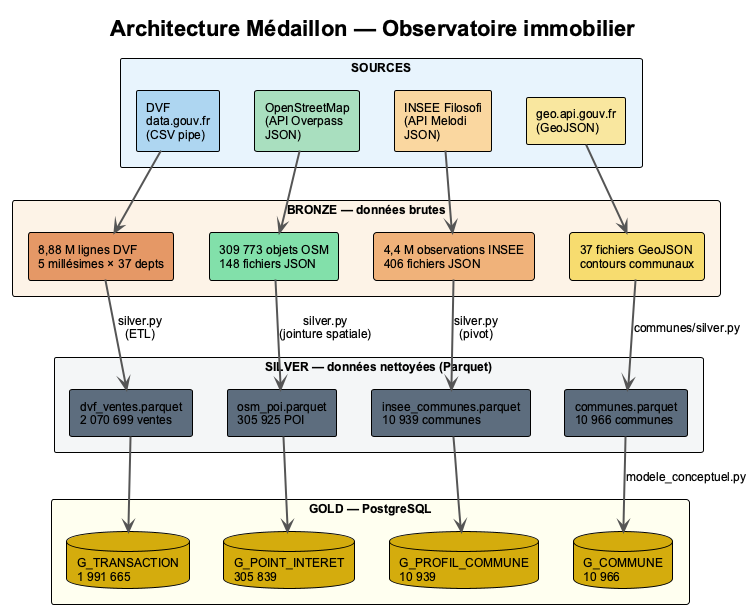
\includegraphics[width=\textwidth]{architecture.png}
\caption{Architecture médaillon -- de l'ingestion au Gold}
\end{figure}

\begin{figure}[H]
\centering
\begin{tabular}{|l|l|l|l|}
\hline
\textbf{Zone} & \textbf{Format} & \textbf{Contenu} & \textbf{Volume} \\
\hline
\textcolor{bronze}{\textbf{Bronze}} & JSON / CSV brut & Données sources téléchargées & \~{}4,6 Go \\
\textcolor{silver}{\textbf{Silver}} & Parquet + PostgreSQL & Données nettoyées & \~{}2,4 M lignes \\
\textcolor{gold}{\textbf{Gold}} & PostgreSQL & 4 tables analytiques & \~{}2,3 M lignes \\
\hline
\end{tabular}
\caption{Synthèse des trois zones du Data Lake}
\end{figure}

\subsection{Justification des formats de stockage}

\begin{description}
  \item[Bronze -- JSON et CSV] Les données sont conservées dans leur format d'origine
  (fichiers tabulaires DVF avec séparateur \texttt{|}, JSON Overpass, JSON API Melodi INSEE).
  Aucune transformation n'est appliquée à ce stade, garantissant la traçabilité.

  \item[Silver -- Parquet] Le format Parquet a été retenu pour sa compression colonaire
  (division par ~5 du volume par rapport au CSV), son typage explicite et son
  interopérabilité avec pandas. Chaque source produit un fichier Parquet unique.

  \item[Gold -- PostgreSQL] Les quatre tables analytiques sont stockées dans PostgreSQL
  pour permettre des requêtes SQL complexes (fenêtres, agrégats, jointures multi-sources),
  l'exposition via une connexion réseau unique et le déploiement sur la plateforme
  universitaire Portainer.
\end{description}

\subsection{Sources de données}

\begin{longtable}{llll}
\toprule
\textbf{Source} & \textbf{Données} & \textbf{Format bronze} & \textbf{Licence} \\
\midrule
DVF -- data.gouv.fr & Transactions 2021--2025 & CSV (\texttt{|}) & CGU DGFiP \\
OpenStreetMap (Overpass) & POI 4 catégories & JSON & ODbL \\
INSEE Filosofi (Melodi) & Indicateurs communes & JSON & Licence Ouverte \\
geo.api.gouv.fr & Contours GeoJSON & GeoJSON & Licence Ouverte \\
BAN & Géocodage (notebook) & API REST & Licence Ouverte \\
\bottomrule
\end{longtable}

% -------------------------------------------------------
%  3. Pipeline ETL
% -------------------------------------------------------
\section{Pipeline ETL -- de Bronze à Gold}

\begin{figure}[H]
\centering
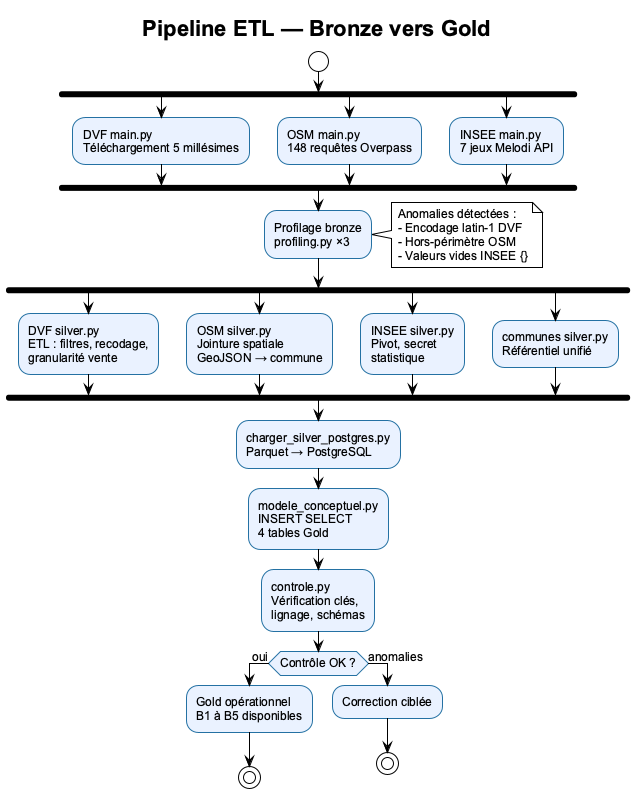
\includegraphics[width=0.75\textwidth]{pipeline.png}
\caption{Flux ETL complet de l'ingestion au Gold}
\end{figure}

\subsection{Étapes du pipeline}

\begin{enumerate}
  \item \textbf{Ingestion Bronze} -- téléchargement des sources dans leur format d'origine
  (\texttt{src/dvf/main.py}, \texttt{src/osm/main.py}, \texttt{src/insee/main.py})
  \item \textbf{Profilage Bronze} -- diagnostic de qualité sur chaque source
  (\texttt{profiling.py} par module, résultats dans \texttt{docs/})
  \item \textbf{Nettoyage Silver} -- transformation et validation
  (\texttt{silver.py} par module + \texttt{src/communes/silver.py})
  \item \textbf{Chargement Silver $\rightarrow$ PostgreSQL} -- via \texttt{src/charger\_silver\_postgres.py}
  \item \textbf{Construction Gold} -- \texttt{src/gold/modele\_conceptuel.py}
  \item \textbf{Contrôle Gold} -- \texttt{src/gold/controle.py}
\end{enumerate}

\subsection{Fédération de données (Polystore)}

Les requêtes Gold réalisent la jointure croisée entre les quatre sources hétérogènes.
La requête B3, par exemple, associe en une seule requête SQL~:

\begin{itemize}[noitemsep]
  \item les transactions DVF (prix, surface)
  \item les POI OSM (transport, équipements, géolocalisation)
  \item les profils INSEE (revenus, population)
  \item le référentiel communal (noms, régions)
\end{itemize}

% -------------------------------------------------------
%  4. Schéma conceptuel Gold
% -------------------------------------------------------
\section{Modèle conceptuel Gold}

\begin{figure}[H]
\centering
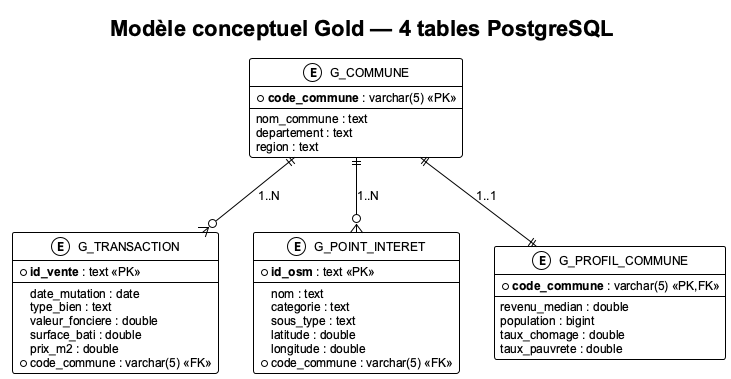
\includegraphics[width=0.85\textwidth]{erd.png}
\caption{Modèle entité-association des 4 tables Gold}
\end{figure}

\subsection{Tables et volumes}

\begin{center}
\begin{tabular}{llr}
\toprule
\textbf{Table} & \textbf{Source Silver} & \textbf{Lignes} \\
\midrule
\texttt{G\_COMMUNE} & \texttt{S\_communes} & 10 966 \\
\texttt{G\_TRANSACTION} & \texttt{S\_dvf\_ventes} & 1 991 665 \\
\texttt{G\_POINT\_INTERET} & \texttt{S\_osm\_poi} & 305 839 \\
\texttt{G\_PROFIL\_COMMUNE} & \texttt{S\_insee\_communes} & 10 939 \\
\bottomrule
\end{tabular}
\end{center}

Tous les contrôles d'intégrité (clés primaires, clés étrangères, schémas, lignage
Silver $\rightarrow$ Gold) sont passés avec 0 anomalie.

% -------------------------------------------------------
%  5. Qualité des données
% -------------------------------------------------------
\section{Qualité des données}

\subsection{DVF -- Transactions immobilières}

\begin{longtable}{p{2.8cm}p{5.5cm}rp{3.5cm}}
\toprule
\textbf{Dimension} & \textbf{Problème} & \textbf{Volume} & \textbf{Correction} \\
\midrule
Exactitude & Encodage double (latin-1 lu comme UTF-8) & Toutes colonnes & Ré-encodage latin-1→UTF-8 \\
Exactitude & Valeurs aberrantes (prix~<~1\,000~€, surface hors [9--1\,000\,m²]) & 3\,336 & Filtres de plausibilité \\
Exactitude & Double saisie (même logement, même jour, prix différents) & 3\,136 & Exclusion \\
Complétude & Lignes éclatées par local/nature de culture & Toutes lignes & Reconstruction 1 vente = 1 ligne \\
Complétude & Transactions sans logement identifiable & \~{}60\% & Maisons/appartements uniquement \\
Cohérence & Codes arrondissements Paris/Lyon ≠ codes INSEE & \~{}8,9\% & 751xx→75056, 6938x→69123 \\
Unicité & Lignes strictement dupliquées & \~{}120\,K/millésime & \texttt{drop\_duplicates()} \\
\bottomrule
\end{longtable}

\subsubsection*{Bilan quantitatif DVF}

\begin{center}
\begin{tabular}{lrr}
\toprule
\textbf{Millésime} & \textbf{Lignes Bronze} & \textbf{Ventes Silver} \\
\midrule
2021 & 2\,020\,967 & 503\,616 \\
2022 & 2\,073\,355 & 485\,638 \\
2023 & 1\,668\,783 & 375\,784 \\
2024 & 1\,524\,087 & 332\,794 \\
2025 & 1\,594\,815 & 372\,867 \\
\midrule
\textbf{Total} & \textbf{8\,882\,007} & \textbf{2\,070\,699} \\
\bottomrule
\end{tabular}
\end{center}

Taux de rétention~: \textbf{23,3\%}. Les 76,7\% restants correspondent aux lignes hors
périmètre (terrains, locaux professionnels, lignes multipropriété).

\subsection{OSM -- Points d'intérêt}

\begin{longtable}{p{2.8cm}p{5.5cm}rp{3.5cm}}
\toprule
\textbf{Dimension} & \textbf{Problème} & \textbf{Volume} & \textbf{Correction} \\
\midrule
Exactitude & Objets hors périmètre (admin\_level manquant) & 311\,210 & Filtre \texttt{admin\_level=6} \\
Exactitude & Auto-écoles, écoles de musique dans la requête «~école~» & 3\,777 & Liste blanche sous-types \\
Exactitude & Tags multi-valeurs séparés par «~;~» & 1\,363 & 1\textsuperscript{re} valeur conservée \\
Exactitude & \texttt{shop=vacant} (locaux vides) & 5\,488 & Flag \texttt{is\_vacant} \\
Complétude & 80\% sans adresse $\Rightarrow$ impossible de rattacher à une commune & \~{}248\,000 & Jointure spatiale GeoJSON \\
Unicité & Doublons aux frontières départementales & 70 & Dédoublonnage sur \texttt{(categorie, id\_osm)} \\
Unicité & Stop\_positions multiples pour un même arrêt & 69\,262→43\,996 & Regroupement par nom + distance~<~100\,m \\
\bottomrule
\end{longtable}

\subsubsection*{Bilan quantitatif OSM}

\begin{center}
\begin{tabular}{lr}
\toprule
\textbf{Étape} & \textbf{Volume} \\
\midrule
Bronze brut & 309\,773 \\
$-$ Hors périmètre éducation & $-$3\,777 \\
$-$ Hors communes ($>$1\,km) & $-$3 \\
$-$ Doublons aux frontières & $-$68 \\
\midrule
\textbf{Silver} & \textbf{305\,925} \\
\bottomrule
\end{tabular}
\end{center}

\subsection{INSEE -- Indicateurs communaux}

\begin{longtable}{p{2.8cm}p{5.5cm}rp{3.5cm}}
\toprule
\textbf{Dimension} & \textbf{Problème} & \textbf{Volume} & \textbf{Correction} \\
\midrule
Exactitude & Valeurs absentes encodées comme objet vide \texttt{\{\}} & 283\,408 obs. & Test sur la clé \texttt{value} \\
Complétude & 25 indicateurs Filosofi non diffusés à l'échelle communale & 25 indicateurs & 2 indicateurs publiables conservés \\
Complétude & Secret statistique sur le taux de pauvreté & 79\% des communes & \texttt{NULL} conservé \\
Cohérence & Code géographique avec millésime (\texttt{2026-COM-35238}) & 10\,939 obs. & Code seul conservé \\
Cohérence & Modalité \texttt{\_T} (total) à ne pas sommer & 9 dimensions & Filtres par modalité \\
\bottomrule
\end{longtable}

\textbf{Bilan~:} 4\,419\,302 observations brutes → \textbf{10\,939 communes × 46 colonnes} en Silver.
Couverture~: revenu médian renseigné pour 88\% des communes.

\subsection{Synthèse des types d'actions correctives}

\begin{center}
\begin{tabular}{lll}
\toprule
\textbf{Type} & \textbf{Source(s)} & \textbf{Exemple} \\
\midrule
Filtrage & DVF, OSM & Prix aberrants, hors périmètre éducation \\
Dédoublonnage & DVF, OSM & Lignes identiques, doublons frontières \\
Recodage & DVF & Arrondissements Paris/Lyon, encodage latin-1 \\
Restructuration & DVF & 1 ligne = 1 vente (reconstruction granularité) \\
Jointure spatiale & OSM & Rattachement communal sans adresse \\
Flagage & DVF, OSM & Reventes <30j, locaux vacants \\
\bottomrule
\end{tabular}
\end{center}

% -------------------------------------------------------
%  6. Dictionnaire de données Gold
% -------------------------------------------------------
\section{Dictionnaire de données -- tables Gold}

\subsection{G\_COMMUNE}
\begin{tabular}{llp{7cm}}
\toprule
\textbf{Colonne} & \textbf{Type} & \textbf{Description} \\
\midrule
\texttt{code\_commune} & varchar(5) & Code INSEE à 5 chiffres -- clé primaire \\
\texttt{nom\_commune} & text & Nom officiel de la commune \\
\texttt{departement} & text & Code département \\
\texttt{region} & text & Région (\texttt{idf}, \texttt{bretagne}, \texttt{occitanie}, \texttt{ara}) \\
\bottomrule
\end{tabular}

\subsection{G\_TRANSACTION}
\begin{tabular}{llp{6.5cm}}
\toprule
\textbf{Colonne} & \textbf{Type} & \textbf{Description} \\
\midrule
\texttt{id\_vente} & text & Identifiant unique -- clé primaire \\
\texttt{date\_mutation} & date & Date de la transaction \\
\texttt{type\_bien} & text & \texttt{Maison} ou \texttt{Appartement} \\
\texttt{valeur\_fonciere} & double & Prix de vente en euros \\
\texttt{surface\_bati} & double & Surface bâtie en m² \\
\texttt{prix\_m2} & double & Prix calculé au m² \\
\texttt{code\_commune} & varchar(5) & FK → \texttt{G\_COMMUNE} \\
\bottomrule
\end{tabular}

\subsection{G\_POINT\_INTERET}
\begin{tabular}{llp{6.5cm}}
\toprule
\textbf{Colonne} & \textbf{Type} & \textbf{Description} \\
\midrule
\texttt{id\_osm} & text & Identifiant OSM -- clé primaire \\
\texttt{nom} & text & Nom de l'établissement (peut être NULL) \\
\texttt{categorie} & text & \texttt{education}, \texttt{sante}, \texttt{commerce}, \texttt{transport} \\
\texttt{sous\_type} & text & Libellé français (ex.~: Lycée / Collège, Pharmacie) \\
\texttt{latitude} & double & Latitude WGS84 \\
\texttt{longitude} & double & Longitude WGS84 \\
\texttt{code\_commune} & varchar(5) & FK → \texttt{G\_COMMUNE} \\
\bottomrule
\end{tabular}

\subsection{G\_PROFIL\_COMMUNE}
\begin{tabular}{llp{6.5cm}}
\toprule
\textbf{Colonne} & \textbf{Type} & \textbf{Description} \\
\midrule
\texttt{code\_commune} & varchar(5) & PK et FK → \texttt{G\_COMMUNE} \\
\texttt{revenu\_median} & double & Revenu médian annuel par unité de consommation (€) \\
\texttt{population} & bigint & Population municipale \\
\texttt{taux\_chomage} & double & Taux de chômage (\%) \\
\texttt{taux\_pauvrete} & double & Taux de pauvreté (seuil 60\%), peut être NULL \\
\bottomrule
\end{tabular}

% -------------------------------------------------------
%  7. Analyses métier B1 à B5
% -------------------------------------------------------
\section{Analyse interactive -- Besoins métier B1 à B5}

\subsection{B1 -- Argumentaire de prix}

\textbf{Situation~:} un négociateur doit défendre le prix d'un bien pendant une visite.

La requête calcule la médiane des médianes annuelles du prix au m² dans la commune
(années $\geq$ 10 ventes). Elle retourne~: médiane, moyenne, Q1, Q3, min, max.

\textbf{Exemple~:} Appartement Paris 11\textsuperscript{e} proposé à 5\,385\,€/m²,
médiane de marché à 9\,812\,€/m² $\Rightarrow$ \textbf{45,1\% sous le marché}.

\subsection{B2 -- Score d'implantation agence}

Score composite (10 meilleures communes par région)~:
$$\text{Score} = 0{,}40 \times \text{dynamique prix} + 0{,}30 \times \text{activité ventes} + 0{,}30 \times \text{équipements}$$

Les trois composantes utilisent \texttt{CUME\_DIST()} pour normaliser les valeurs sur [0, 1]
dans leur région, rendant les 4 régions comparables.

\subsection{B3 -- Recherche logement autour du travail}

La requête croise DVF (prix biens comparables), OSM (accessibilité) et INSEE (profil).
Le \texttt{ratio\_prix\_revenu\_annuel} mesure l'effort financier~: un ratio de 8 = 8 années
de salaire brut.

\subsection{B4 -- Tendance du marché}

Utilise \texttt{LAG()} et \texttt{generate\_series()} pour une série temporelle complète
2021--2025. Verdict~: hausse / stable / baisse / non\_concluante ($\pm$3\%).

\textbf{Exemple~:} Lyon Appartement~: \textbf{baisse} ($-$12,5\% sur 5 ans).

\subsection{B5 -- Zones sous-évaluées}

Filtre les communes~: prix médian $<$ seuil régional (90\%), score équipements $>$ 60/100,
revenu médian positif. Ce dernier critère écarte les zones simplement pauvres.

% -------------------------------------------------------
%  8. Déploiement
% -------------------------------------------------------
\section{Déploiement}

\subsection{Image Docker}

L'image est publiée sur Docker Hub~: \texttt{rayanhcm0/datalake-immo:latest}.
Elle est compilée en \texttt{linux/amd64} depuis Apple Silicon avec \texttt{docker buildx}.

\begin{lstlisting}[language=bash]
docker run --env-file .env -p 8888:8888 rayanhcm0/datalake-immo:latest
\end{lstlisting}

Accès au notebook~: \texttt{http://localhost:8888} -- mot de passe~: \texttt{cleenmain2025}

\subsection{Portainer -- plateforme universitaire}

Le container est déployé sur la plateforme Docker de l'université.
La connexion PostgreSQL est configurée via la variable d'environnement \texttt{DATABASE\_URL}.
Les tables Silver et Gold sont déjà peuplées ; le notebook s'exécute sans ré-ingestion.

% -------------------------------------------------------
%  9. Conclusion
% -------------------------------------------------------
\section{Conclusion}

Ce projet met en œuvre une architecture Data Lake complète~:

\begin{itemize}
  \item \textbf{3 sources hétérogènes} intégrées (fichiers plats, API JSON, données spatiales)
  \item \textbf{Architecture médaillon} Bronze / Silver / Gold avec justification des formats
  \item \textbf{6 types d'actions correctives} documentées et quantifiées
  \item \textbf{Fédération polystore} réalisée en SQL sur 4 tables issues de sources distinctes
  \item \textbf{5 analyses métier complexes} paramétrables et opérationnelles
  \item \textbf{Déploiement Docker} sur la plateforme universitaire
\end{itemize}

L'ensemble du pipeline est reproductible depuis les scripts fournis. Le notebook
\texttt{analyse\_immo.ipynb} constitue le démonstrateur interactif final.

\end{document}
